%\documentclass[a4paper,12pt,oneside]{llncs}
\documentclass[12pt,letterpaper]{report}
\usepackage[right=2cm,left=3cm,top=2cm,bottom=2cm,headsep=0cm]{geometry}

%%%%%%%%%%%%%%%%%%%%%%%%%%%%%%%%%%%%%%%%%%%%%%%%%%%%%%%%%%%
%% Juego de caracteres usado en el archivo fuente: UTF-8
\usepackage{ucs}
\usepackage[utf8x]{inputenc}

%%%%%%%%%%%%%%%%%%%%%%%%%%%%%%%%%%%%%%%%%%%%%%%%%%%%%%%%%%%
%% Juego de caracteres usado en la salida dvi
%% Otra posibilidad: \usepackage{t1enc}
\usepackage[T1]{fontenc}

%%%%%%%%%%%%%%%%%%%%%%%%%%%%%%%%%%%%%%%%%%%%%%%%%%%%%%%%%%%
%% Ajusta maergenes para a4
%\usepackage{a4wide}

%%%%%%%%%%%%%%%%%%%%%%%%%%%%%%%%%%%%%%%%%%%%%%%%%%%%%%%%%%%
%% Uso fuente postscript times, para que los ps y pdf queden y pequeños...
\usepackage{times}

%%%%%%%%%%%%%%%%%%%%%%%%%%%%%%%%%%%%%%%%%%%%%%%%%%%%%%%%%%%
%% Posibilidad de hipertexto (especialmente en pdf)
%\usepackage{hyperref}
\usepackage[bookmarks = true, colorlinks=true, linkcolor = black, citecolor = black, menucolor = black, urlcolor = black]{hyperref}

%%%%%%%%%%%%%%%%%%%%%%%%%%%%%%%%%%%%%%%%%%%%%%%%%%%%%%%%%%%
%% Graficos 
\usepackage{graphics,graphicx}

%%%%%%%%%%%%%%%%%%%%%%%%%%%%%%%%%%%%%%%%%%%%%%%%%%%%%%%%%%%
%% Ciertos caracteres "raros"...
\usepackage{latexsym}

%%%%%%%%%%%%%%%%%%%%%%%%%%%%%%%%%%%%%%%%%%%%%%%%%%%%%%%%%%%
%% Matematicas aun más fuertes (american math dociety)
\usepackage{amsmath}

%%%%%%%%%%%%%%%%%%%%%%%%%%%%%%%%%%%%%%%%%%%%%%%%%%%%%%%%%%%
\usepackage{multirow} % para las tablas
\usepackage[spanish,es-tabla]{babel}

%%%%%%%%%%%%%%%%%%%%%%%%%%%%%%%%%%%%%%%%%%%%%%%%%%%%%%%%%%%
%% Fuentes matematicas lo mas compatibles posibles con postscript (times)
%% (Esto no funciona para todos los simbolos pero reduce mucho el tamaño del
%% pdf si hay muchas matamaticas....
\usepackage{mathptm}

%%% VARIOS:
\usepackage{slashbox}
\usepackage{array}
\usepackage{listings}
\usepackage{multirow}

%% MARCA DE AGUA
%% Este package de "draft copy" NO funciona con pdflatex
%%\usepackage{draftcopy}
%% Este package de "draft copy" SI funciona con pdflatex
%%%\usepackage{pdfdraftcopy}
%%%%%%%%%%%%%%%%%%%%%%%%%%%%%%%%%%%%%%%%%%%%%%%%%%%%%%%%%%%
%% Indenteacion en español...
\usepackage[spanish]{babel}
\usepackage{listings}
% Para escribir código en C
% \begin{lstlisting}[language=C]
% #include <stdio.h>
% int main(int argc, char* argv[]) {
% puts("Hola mundo!");
% }
% \end{lstlisting}


\title{SendUCA}
\author{Grupo 1 PINF}

\begin{document}
	\maketitle
	\thispagestyle{empty}
	\newpage
	\tableofcontents
	%%\listoftables
	%%\newpage
	
	%%\listoffigures
	%%\newpage
	
	%%%% REAL WORK BEGINS HERE:
	
	%%Configuracion del paquete listings
	\lstset{language=bash, numbers=left, numberstyle=\tiny, numbersep=10pt, firstnumber=1, stepnumber=1}
	
\chapter{Prolegómeno}		
\section{Introducción}
	\subsection{Motivación}
		\noindent 1º Motivación\\
		La motivación para la creación de este proyecto es crear el software necesario
		para realizar con exito la asignatura de la que deriva. Esta asignatura es Proyectos Informáticos.
		\\~\\
		\noindent 2º Motivación\\
		Por otra parte, la otra motivación, es poder ganar la competición y conseguir
		una oferta de trabajo.
	\subsection{Descripción del sistema actual}
		El Sistema actual, permite realizar una votación programada, añadiendole un censo, un horario
		y una rectificación de voto.
		\\~\\
		También, dicho sistema, permite modificar todas las propiedades de los usuarios y exportar/importar
		dichos usuarios a un formato de carga masiva (csv).
		\\~\\
		Por otra parte, se permite actualmente el acceso de forma remota (sin entorno local) y con verificación
		con certificado SSL.
		\\~\\
		Para más información de esto mismo, consultesé la dirección \href{https://senuca.herokuapp.com/}{SenUca}.
	\subsection{Objetivos y alcance del proyecto}
		\noindent Objetivos\\
		\\~\\
		Los objetivos del proyecto son los siguientes:
		\begin{enumerate}
			\item Crear un software con autenticación segura para acceder a las votaciones.
			\item Crear votaciones, añadirles participantes y obtener un resumen de la misma una vez acabe.
			\item Crear una buena cohesión del equipo para garantizar el mejor resultado posible.
			\item Garantizar, incluso al más bajo nivel, que todos los datos de los usuarios de la aplicación estén seguros y estables.
			\item Crear una documentación lo suficientemente exhaustiva para que el mismo equipo u otro más adelante, prosiga con la labor sin problemas.
		\end{enumerate}
		\noindent Alcance\\
		\\~\\
		El alcance esperado de este proyecto es cumplir todos los objetivos y presentar un proyecto digno de un equipo de ingeniería informática.
	\subsection{Organización del documento}
		Este documento se divide en 3 capítulos, que se detallan a continuación:
		\begin{enumerate}
			\item Capítulo 1: En este capítulo se desarrolla la introducción del proyecto entero, así como
			      objetivos planteados, el alcance de los mismos y la propia organización del proyecto.
			\item Capítulo 2: En este capítulo se desarrolla el centro del proyecto. Aquí es donde se especifica 
				  es lo que se ha hecho en el producto software y como se ha hecho.
			\item Capítulo 3: En este capítulo se desarrolla el epílogo del proyecto, donde se puede ver claramente
				  un manual de usuario, instalación del producto software y unas conclusiones del equipo sobre el
				  desarrollo del proyecto.
		\end{enumerate}
\section{Planificación}
	\subsection{Metodología de desarrollo}
		\noindent Scrum\\
		\\~\\
		Como se puede apreciar con el título de este párrafo, hemos seguido la metodología de desarrollo Scrum.
		En concreto, la variante de Prototipos.
		\\~\\
	\subsection{Planificación}
		\noindent Sprints\\
		\\~\\
		Como buen derivado de Scrum, la metodología de Prototipos tiene asociado a cada prototipo un Sprint.
		En concreto, en este proyecto, se han planificado 5 Sprints:
		\\~\\
		\begin{enumerate}
			\item Sprint 1: Del ​11/11/2019​ al ​17/11/2019.
			\begin{itemize}
				\item Dedicado a empezar a andar en el proyecto, aunque sea en local.
				\item Crear mockups de diseño y su posterior implementación en html y css.
				\item Análisis principal del proyecto ('que hace').
			\end{itemize}
			\item Sprint 2: Del ​18/11/2019​ al ​24/11/2019.
			\begin{itemize}
				\item Dedicado a crear lógica principal del core del sistema.
				\item Creación de la mayoría de las vistas de la aplicación.
				\item Análisis de la lógica principal de la aplicación y descripción exhaustiva de lo mismo.
			\end{itemize}
			\item Sprint 3: Del ​25/11/2019​ al ​8/12/2019.
			\begin{itemize}
				\item Dedicado a crear la mayoría de la lógica de la aplicación.
				\item Adaptación de las vistas al entorno de programación real.
				\item Análisis de la mayoría de la lógica de la aplicación y descripción exhaustiva de lo mismo..
			\end{itemize}
			\item Sprint 4: Del ​8/12/2019​ al ​20/12/2019.
			\begin{itemize}
				\item Dedicado a retocar pequeños bugs de lógica de la aplicación.
				\item Creación de vistas “responsives” de la aplicación.
			\end{itemize}
			\item Sprint 5: Del ​8/1/2020​ al ​20/1/2019​.
			\begin{itemize}
				\item Testing de la aplicación a nivel de test unitarios.
				\item Testing de la aplicación a nivel de test de integración.
			\end{itemize}
			\item Diagrama de Gantt
				\\~\\
				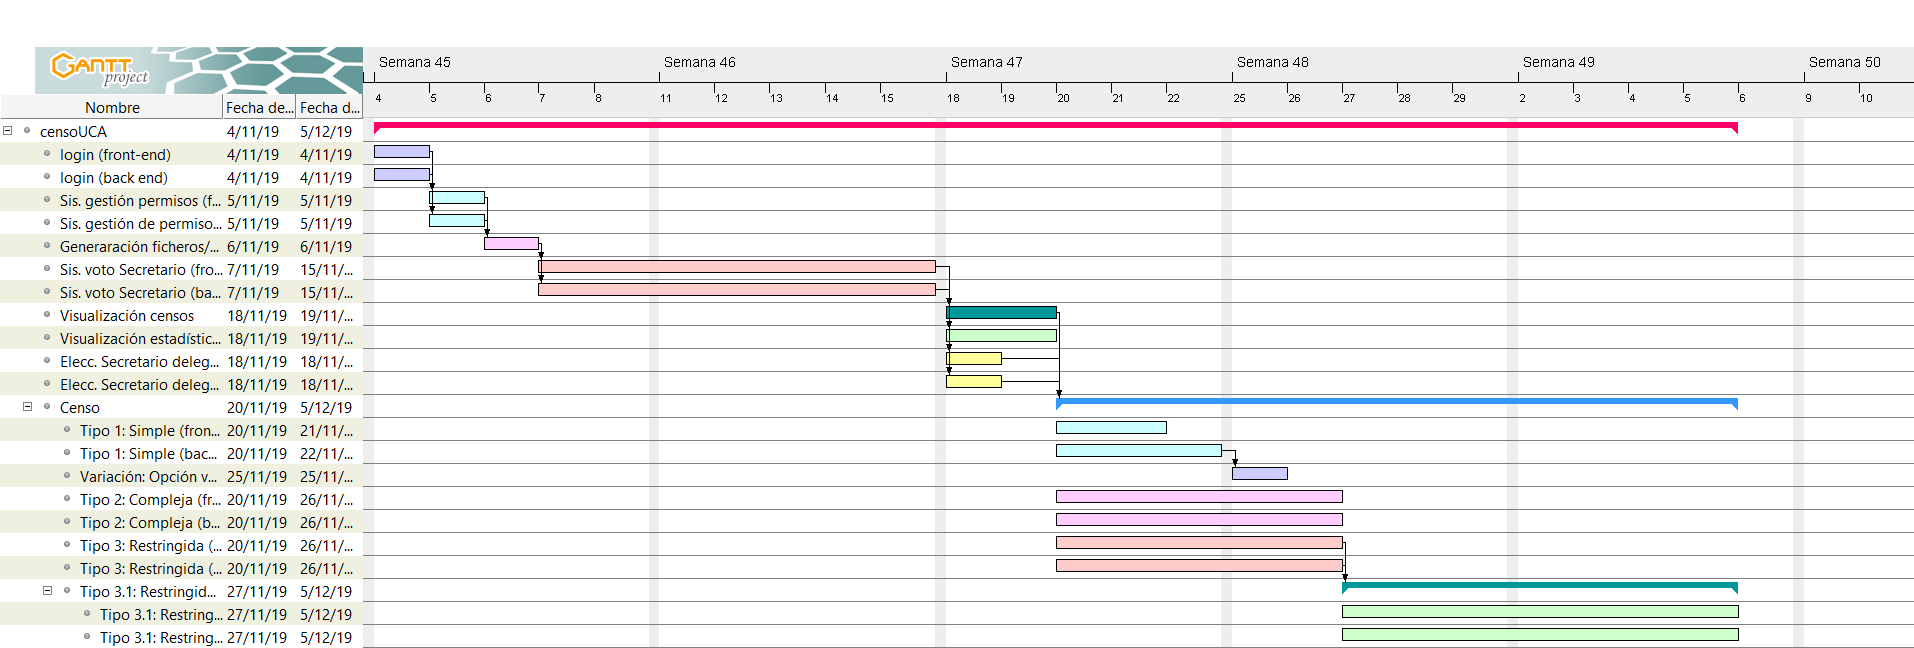
\includegraphics[width=\textwidth]{diagrama_base}
		\end{enumerate}
\chapter{Desarrollo}
\section{Análisis de requisitos}
	\subsection{Objetivos del sistema}
		\noindent Controlar el acceso al sistema\\
		Descripción: El sistema deberá gestionar el acceso a la aplicación, restringiendo el mismo a personas registradas en el sistema y autentificando las credenciales del usuario.
		\\~\\
		Realizar votaciones\\
		Descripción: El sistema deberá permitir la creación y la participación de los usuarios del sistema en votaciones, en base al cumplimiento de unas pre condiciones específicas.
		\\~\\
		Realizar Elecciones \\
		Descripción: 
		El sistema deberá permitir la creación y la participación de los usuarios del sistema en elecciones, en base al cumplimiento de unas pre condiciones específicas.
		\\~\\ 
		Realizar Consultas\\
		Descripción: El sistema deberá permitir configurar la creación de una votación / elección como una consulta.
		\\~\\  
		Mostrar Estadísticas\\
		Descripción: El sistema deberá ser capaz de mostrar estadísticas referentes a cada votación / elección / consulta que se realice.\\   
		
	\subsection{Catálogo de actores}
		\noindent Administrador\\
		Descripción: Se encarga de la asignación de permisos al resto de usuarios, velar por la integridad del sistema, etc. Este rol lo pueden desempeñar una persona o varias, con distintas claves de acceso.
		\\~\\
		Elector\\
		Descripción: Cada uno de los usuarios incluidos en el censo de una elección/votación y que tiene derecho al voto en la misma.
		\\~\\
		Secretario\\
		Descripción: Son los encargados de dar de alta los procesos electorales, fijando las características de los mismos como censo, calendarios, etc.
		\\~\\
		Secretario general\\
		Descripción: En algunos procesos electorales los secretarios[ACT-003] pueden delegar parte de sus funciones en los secretarios delegados. También el administrador[ACT-001] puede crear esta figura, en el caso de ausencia de los secretarios.
		\\~\\
		
	\subsection{Requisitos funcionales}
	
		\begin{table}[htp]
			\resizebox{.8\textwidth}{!}{
			\begin{tabular}{|c|c|}
				\hline
				UC-0001          & Iniciar Sesión                                                                                                                                                                                                                                                                                                                                                                                                                \\ \hline
				Descripción      & \begin{tabular}[l]{@{}l@{}}El sistema deberá comportarse tal como se describe \\ en el siguiente caso de uso cuando algún usuario \\ desee iniciar sesión para acceder al sistema.\end{tabular}                                                                                                                                                                                                                               \\ \hline
				Precondición     & Usuario sin iniciar sesión.                                                                                                                                                                                                                                                                                                                                                                                                   \\ \hline
				Secuencia normal & \begin{tabular}[l]{@{}l@{}}1.El sistema muestra la pantalla para iniciar sesión.\\ 2.El usuario introduce sus datos en la pantalla.\\ 3.El sistema verifica que los datos son correctos y muestra \\ la pantalla principal asociada al rol del usuario.\end{tabular}                                                                                                                                                          \\ \hline
				Postcondición    & Usuario con sesión iniciada.                                                                                                                                                                                                                                                                                                                                                                                                  \\ \hline
				Excepciones      & \begin{tabular}[l]{@{}l@{}}1.Si el usuario ya no desea loguearse, el usuario cancela\\  el inicio de sesión, a continuación este caso de uso queda sin efecto.\\ 2.Si el usuario no existe, el sistema mostrará un mensaje\\  de error, a continuación este caso de uso queda sin efecto.\\ 3.Si los datos son incorrectos, el sistema mostrará un\\ mensaje de error, a continuación este caso de uso continúa.\end{tabular} \\ \hline
				Comentarios      & Ninguno                                                                                                                                                                                                                                                                                                                                                                                                                       \\ \hline
			\end{tabular}}
		\end{table}
		\hspace{2em}
		\begin{table}[htp]
			\resizebox{.8\textwidth}{!}{
			\begin{tabular}{|c|c|}
				\hline
				UC-0002          & Crear Votación                                                                                                                                                                                                                                                                                            \\ \hline
				Descripción      & \begin{tabular}[l]{@{}l@{}}El sistema deberá comportarse tal como se describe \\ en el siguiente caso de uso cuando algún usuario con los permisos \\ oportunos desee crear una votación.\end{tabular}                                                                                                    \\ \hline
				Precondición     & Usuario previamente logueado.                                                                                                                                                                                                                                                                             \\ \hline
				Secuencia normal & \begin{tabular}[l]{@{}l@{}}1.El sistema muestra la pantalla para crear una votación.\\ 2.El usuario establece los datos de creación\\  asociados a la votación.\\ 3.El sistema verifica que los datos son correctos y muestra un mensaje de\\  éxito indicando que la votación se ha creado.\end{tabular} \\ \hline
				Postcondición    & Votación generada exitosamente.                                                                                                                                                                                                                                                                           \\ \hline
				Excepciones      & \begin{tabular}[l]{@{}l@{}}1.Si el usuario ya no desea crear la votación, el usuario cancela \\ la creación, a continuación este caso de uso queda sin efecto.\\ 2.Si los datos son incorrectos, el sistema mostrará un mensaje de \\ error, a continuación este caso de uso continúa.\end{tabular}       \\ \hline
				Comentarios      & Ninguno                                                                                                                                                                                                                                                                                                   \\ \hline
			\end{tabular}}
		\end{table}
		\hspace{2em}
		\begin{table}[htp]
			\resizebox{.8\textwidth}{!}{
			\begin{tabular}{|c|c|}
				\hline
				UC-0003          & Crear Elección                                                                                                                                                                                                                                                                                         \\ \hline
				Descripción      & \begin{tabular}[l]{@{}l@{}}El sistema deberá comportarse tal como se describe \\ en el siguiente caso de uso cuando algún usuario con los\\  permisos oportunos desee crear una elección.\end{tabular}                                                                                                 \\ \hline
				Precondición     & Usuario previamente logueado.                                                                                                                                                                                                                                                                          \\ \hline
				Secuencia normal & \begin{tabular}[l]{@{}l@{}}1.El sistema muestra la pantalla para crear una elección.\\ 2.El usuario establece los datos de creación asociados a la elección.\\ 3.El sistema verifica que los datos son correctos y muestra un\\  mensaje de éxito indicando que la elección se ha creado.\end{tabular} \\ \hline
				Postcondición    & Elección generada exitosamente.                                                                                                                                                                                                                                                                        \\ \hline
				Excepciones      & \begin{tabular}[l]{@{}l@{}}1.Si el usuario ya no desea crear la elección, el usuario cancela \\ la creación, a continuación este caso de uso queda sin efecto.\\ 2.Si los datos son incorrectos, el sistema mostrará un mensaje de \\ error, a continuación este caso de uso continúa.\end{tabular}    \\ \hline
				Comentarios      & Ninguno                                                                                                                                                                                                                                                                                                \\ \hline
			\end{tabular}}
		\end{table}
		\hspace{2em}
		\begin{table}[htp]
			\resizebox{.8\textwidth}{!}{
			\begin{tabular}{|c|c|}
				\hline
				UC-0004          & Crear Consulta                                                                                                                                                                                             \\ \hline
				Descripción      & \begin{tabular}[l]{@{}l@{}}El sistema deberá comportarse tal como se describe en \\ el siguiente caso de uso cuando algún usuario con los permisos \\ oportunos desee crear una consulta.\end{tabular}     \\ \hline
				Precondición     & \begin{tabular}[l]{@{}l@{}}Usuario previamente logueado y realizando la creación \\ de una votación / elección.\end{tabular}                                                                               \\ \hline
				Secuencia normal & \begin{tabular}[l]{@{}l@{}}1.El sistema muestra la opción para la generación\\  de una consulta.\\ 2.El usuario selecciona la opción de generar una\\  votación / elección como una consulta.\end{tabular} \\ \hline
				Postcondición    & Votación / Elección generada exitósamente como una Consulta.                                                                                                                                               \\ \hline
				Excepciones      & \begin{tabular}[l]{@{}l@{}}Si el usuario ya no desea crear la votación / elección como\\  una consulta, el usuario desmarca la opción,  a continuación \\ \\ este caso de uso continúa.\end{tabular}       \\ \hline
				Comentarios      & \begin{tabular}[l]{@{}l@{}}En caso de cumplirse la excepción, se creará una votación\\  o una elección, definidos sus casos de uso\\  respectivamente en UC-0003 y UC-0004\\ .\end{tabular}                \\ \hline
			\end{tabular}}
		\end{table}
		\hspace{2em}
		\begin{table}[htp]
			\resizebox{.8\textwidth}{!}{
			\begin{tabular}{|c|c|}
				\hline
				UC-0005          & Participar en Votación Simple                                                                                                                                                                                                                                                                                                   \\ \hline
				Descripción      & \begin{tabular}[l]{@{}l@{}}El sistema deberá comportarse tal como se describe en el \\ siguiente caso de uso cuando algún usuario desee participar\\  en una votación de tipo simple.\end{tabular}                                                                                                                              \\ \hline
				Precondición     & \begin{tabular}[l]{@{}l@{}}Usuario logueado y con permisos para participar en una\\  votación de tipo simple.\end{tabular}                                                                                                                                                                                                      \\ \hline
				Secuencia normal & \begin{tabular}[l]{@{}l@{}}1.El sistema muestra la pantalla para participar en la votación.\\ 2.El sistema muestra la pregunta, y las opciones de la votación\\  (a favor, en contra, abstención).\\ 3.El usuario lee la pregunta, y selecciona la opción deseada.\\ 4.El sistema recoge los datos de la votación.\end{tabular} \\ \hline
				Postcondición    & Usuario participa exitosamente en la votación simple.                                                                                                                                                                                                                                                                           \\ \hline
				Excepciones      & \begin{tabular}[l]{@{}l@{}}1.Si el usuario ya no desea votar, el usuario cancela su \\ votación, a continuación este caso de uso queda sin efecto.\\ 2.Si el usuario no selecciona una opción, el sistema mostrará un\\  mensaje de error, a continuación este caso de uso continúa.\end{tabular}                               \\ \hline
				Comentarios      & Ninguno.                                                                                                                                                                                                                                                                                                                        \\ \hline
			\end{tabular}}
		\end{table}
		\hspace{2em}
		\begin{table}[htp]
			\resizebox{.8\textwidth}{!}{
			\begin{tabular}{|c|c|}
				\hline
				UC-0006          & Participar en Votación Compleja                                                                                                                                                                                                                                                                                     \\ \hline
				Descripción      & \begin{tabular}[l]{@{}l@{}}El sistema deberá comportarse tal como se describe en el \\ siguiente caso de uso cuando algún usuario desee participar\\  en una votación de tipo compleja.\end{tabular}                                                                                                                \\ \hline
				Precondición     & \begin{tabular}[l]{@{}l@{}}Usuario logueado y con permisos para participar en\\ una votación de tipo compleja.\end{tabular}                                                                                                                                                                                         \\ \hline
				Secuencia normal & \begin{tabular}[l]{@{}l@{}}1.El sistema muestra la pantalla para participar en la votación.\\ 2.El sistema muestra la pregunta, y las opciones de la votación (\\ múltiples opciones).\\ 3.El usuario lee la pregunta, y selecciona la opción deseada.\\ 4.El sistema recoge los datos de la votación.\end{tabular} \\ \hline
				Postcondición    & Usuario participa exitosamente en la votación compleja.                                                                                                                                                                                                                                                             \\ \hline
				Excepciones      & \begin{tabular}[l]{@{}l@{}}1.Si el usuario ya no desea votar, el usuario cancela su \\ votación, a continuación este caso de uso queda sin efecto.\\ 2.Si el usuario no selecciona una opción, el sistema mostrará un\\  mensaje de error, a continuación este caso de uso continúa.\end{tabular}                   \\ \hline
				Comentarios      & Ninguno.                                                                                                                                                                                                                                                                                                            \\ \hline
			\end{tabular}}
		\end{table}
		\hspace{2em}
		\begin{table}[htp]
			\resizebox{.8\textwidth}{!}{
			\begin{tabular}{|c|c|}
				\hline
				UC-0007          & Participar en Elecciones Unipersonales                                                                                                                                                                                                                                                            \\ \hline
				Descripción      & \begin{tabular}[l]{@{}l@{}}El sistema deberá comportarse tal como se describe en el\\  siguiente caso de uso cuando algún usuario desee\\  participar en una elección a cargos unipersonales.\end{tabular}                                                                                        \\ \hline
				Precondición     & \begin{tabular}[l]{@{}l@{}}Usuario logueado y con permisos para participar en una \\ \\ elección a cargos unipersonale.\end{tabular}                                                                                                                                                              \\ \hline
				Secuencia normal & \begin{tabular}[l]{@{}l@{}}1.El sistema muestra la pantalla para participar en la elección.\\ 2.El sistema muestra los candidatos elegibles.\\ 3.El usuario lee la información de los candidatos, y selecciona\\  la opción deseada.\\ 4.El sistema recoge los datos de la elección.\end{tabular} \\ \hline
				Postcondición    & Usuario participa exitosamente en la elección a cargos unipersonales.                                                                                                                                                                                                                             \\ \hline
				Excepciones      & \begin{tabular}[l]{@{}l@{}}1.Si el usuario ya no desea votar, el usuario cancela su \\ elección, a continuación este caso de uso queda sin efecto.\\ 2.Si el usuario no selecciona una opción, el sistema mostrará un \\ mensaje de error, a continuación este caso de uso continúa.\end{tabular} \\ \hline
				Comentarios      & Ninguno.                                                                                                                                                                                                                                                                                          \\ \hline
			\end{tabular}}
		\end{table}
		\hspace{2em}
		\begin{table}[htp]
			\resizebox{.8\textwidth}{!}{
			\begin{tabular}{|c|c|}
				\hline
				UC-0008          & Participar en Elecciones por Grupos                                                                                                                                                                                                                                                                  \\ \hline
				Descripción      & \begin{tabular}[l]{@{}l@{}}El sistema deberá comportarse tal como se describe en el\\  siguiente caso de uso cuando algún usuario desee\\  participar en una elección por grupos.\end{tabular}                                                                                                       \\ \hline
				Precondición     & \begin{tabular}[l]{@{}l@{}}Usuario logueado y con permisos para participar \\ en una elección por grupos.\end{tabular}                                                                                                                                                                               \\ \hline
				Secuencia normal & \begin{tabular}[l]{@{}l@{}}1.El sistema muestra la pantalla para participar en la \\ elección.\\ 2.El sistema muestra los candidatos elegibles.\\ 3.El usuario lee la información de los candidatos, y selecciona\\  la opción deseada.\\ 4.El sistema recoge los datos de la elección.\end{tabular} \\ \hline
				Postcondición    & Usuario participa exitosamente en la elección por grupos.                                                                                                                                                                                                                                            \\ \hline
				Excepciones      & \begin{tabular}[l]{@{}l@{}}1.Si el usuario ya no desea votar, el usuario cancela su elección, \\ a continuación este caso de uso queda sin efecto.\\ 2.Si el usuario no selecciona una opción, el sistema\\  mostrará un mensaje de error, a \\ continuación este caso de uso continúa.\end{tabular} \\ \hline
				Comentarios      & Ninguno.                                                                                                                                                                                                                                                                                             \\ \hline
			\end{tabular}}
		\end{table}
		\hspace{2em}
		\begin{table}[htp]
			\resizebox{.8\textwidth}{!}{
			\begin{tabular}{|c|c|}
				\hline
				UC-0009          & Mostrar Estadísticas                                                                                                                                                                                                         \\ \hline
				Descripción      & \begin{tabular}[l]{@{}l@{}}El sistema deberá comportarse tal como se describe en el siguiente \\ caso de uso cuando algún usuario desee ver las estadísticas asociadas\\  a una votación / elección / consulta.\end{tabular} \\ \hline
				Precondición     & Usuario logueado y votación / elección / consulta previamente concluída.                                                                                                                                                     \\ \hline
				Secuencia normal & \begin{tabular}[l]{@{}l@{}}1.El usuario selecciona la opción de mostrar estadísticas.\\ 2.El sistema muestra los datos estadísticos asociados a la\\  votación / elección / consulta.\end{tabular}                           \\ \hline
				Postcondición    & Estadísticas visualizadas exitosamente                                                                                                                                                                                       \\ \hline
				Excepciones      & \begin{tabular}[l]{@{}l@{}}Si no se ha realizado ninguna votación / elección / consulta, el\\  sistema mostrará un mensaje de error, a continuación este caso \\ de uso queda sin efecto.\end{tabular}                       \\ \hline
				Comentarios      & Ninguno.                                                                                                                                                                                                                     \\ \hline
			\end{tabular}}
		\end{table}
	
	\subsection{Modelos estáticos del sistema}

		\subsubsection{Modelo Estático de los Procesos Electorales.}
			\begin{figure}[htp]
				\centering
				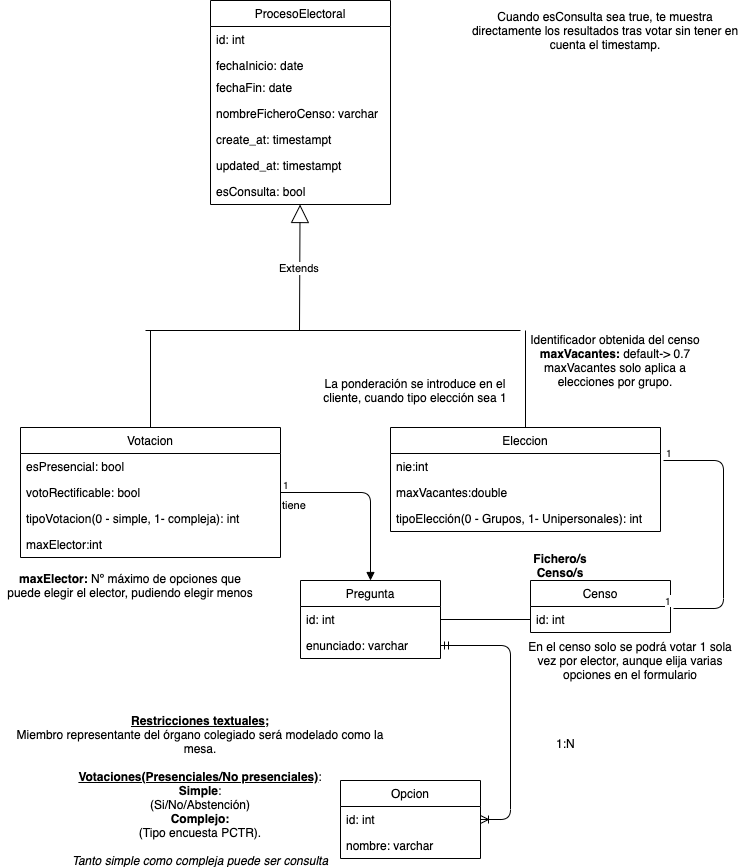
\includegraphics[width=0.9\linewidth]{img/MEProcesosElectorales}
				\caption{}
				\label{fig:meprocesoselectorales}
			\end{figure}
		\newpage
		
		\subsubsection{Modelo Estático de la jerarquía de usuarios del Sistema}
			\begin{figure}[htp]
				\centering
				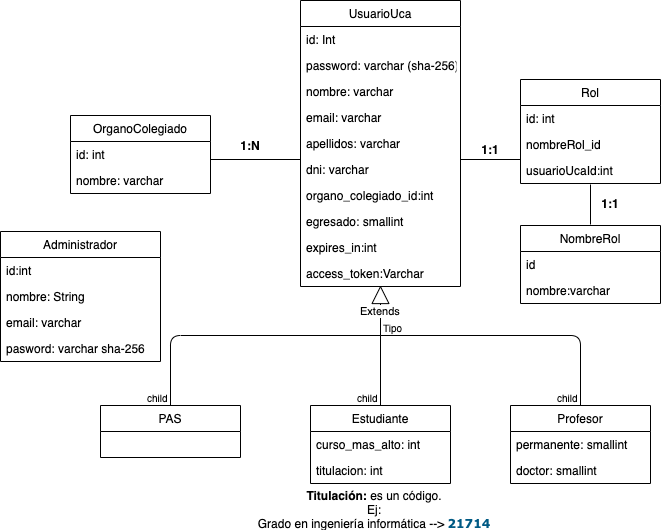
\includegraphics[width=0.9\linewidth]{img/MEJerarquiaUsuarios}
				\caption{}
				\label{fig:meprocesoselectorales}
			\end{figure}
		\newpage	
	\subsection{Requisitos de información}
		\subsubsection{Requsitos de Información de Usuarios}
		\begin{table}[htp]
			\resizebox{.8\textwidth}{!}{
			\begin{tabular}{|c|c|}
				\hline
				IRQ - 0001                        & UsuarioUca                                                                                                                                                                                                                                                                                                                           \\ \hline
				Versión                           & 1.0                                                                                                                                                                                                                                                                                                                                  \\ \hline
				Autores                           & \begin{tabular}[c]{@{}c@{}}José Joaquín Pérez-Calderón Ortiz\\ José Javier Gómez Rosado\\ Pablo Pastor Muñoz\\ Pablo Rodríguez Gómez\\ Francisco Javier Jiménez Vázquez\end{tabular}                                                                                                                                                 \\ \hline
				Datos Específicos                 & \begin{tabular}[c]{@{}c@{}}Identificador\\ Contraseña\\ Nombre\\ Email\\ Apellidos\\ DNI\\ Órgano Colegiado al que pertenece\\ Egresado(Sí/No)\\ Campo de expiración de clave\\ Identificador de acceso\end{tabular}                                                                                                                 \\ \hline
				Descripción                       & \begin{tabular}[c]{@{}c@{}}El sistema deberá almacenar la información\\  relacionada a cada usuario de la UCA\end{tabular}                                                                                                                                                                                                           \\ \hline
				Importancia                       & Vital                                                                                                                                                                                                                                                                                                                                \\ \hline
				Estado                            & Hecho                                                                                                                                                                                                                                                                                                                                \\ \hline
				\multicolumn{1}{|l|}{Comentarios} & \multicolumn{1}{l|}{\begin{tabular}[c]{@{}l@{}}Al no contar con el servicio web de verificación LDAP, hemos\\  modelado los usuarios del sistema de forma temporal. \\ En un futuro se puede desplegar utilizando cualquier framework \\ de autenticación. El subconjunto administrador está incluido en \\ esta tabla\end{tabular}} \\ \hline
			\end{tabular}}
		\end{table}
		
		\begin{table}[htp]
			\resizebox{.8\textwidth}{!}{
			\begin{tabular}{|c|c|}
				\hline
				IRQ - 0002                        & Rol                                                                                                                                                                                            \\ \hline
				Versión                           & 1.0                                                                                                                                                                                            \\ \hline
				Autores                           & \begin{tabular}[c]{@{}c@{}}José Joaquín Pérez-Calderón Ortiz\\ José Javier Gómez Rosado\\ Pablo Pastor Muñoz\\ Pablo Rodríguez Gómez\\ Francisco Javier Jiménez Vázquez\end{tabular}           \\ \hline
				Datos Específicos                 & \begin{tabular}[c]{@{}c@{}}Identificador\\ Identificador del nombre del rol\\ Identificador de usuario de la UCA\end{tabular}                                                                  \\ \hline
				Descripción                       & El sistema deberá almacenar los identificadores de los roles.                                                                                                                                  \\ \hline
				Importancia                       & Vital                                                                                                                                                                                          \\ \hline
				Estado                            & Hecho                                                                                                                                                                                          \\ \hline
				\multicolumn{1}{|l|}{Comentarios} & \multicolumn{1}{l|}{\begin{tabular}[c]{@{}l@{}}Se crea una nueva entidad para evitar la incorrecta introducción\\  de valores así como la generación de inconsistencias de datos\end{tabular}} \\ \hline
			\end{tabular}}
		\end{table}

		\begin{table}[htp]
			\resizebox{.8\textwidth}{!}{
			\begin{tabular}{|c|c|}
				\hline
				IRQ - 0003                        & NombreRol                                                                                                                                                                            \\ \hline
				Versión                           & 1.0                                                                                                                                                                                  \\ \hline
				Autores                           & \begin{tabular}[c]{@{}c@{}}José Joaquín Pérez-Calderón Ortiz\\ José Javier Gómez Rosado\\ Pablo Pastor Muñoz\\ Pablo Rodríguez Gómez\\ Francisco Javier Jiménez Vázquez\end{tabular} \\ \hline
				Datos Específicos                 & \begin{tabular}[c]{@{}c@{}}Identificador\\ Nombre del Rol.\end{tabular}                                                                                                              \\ \hline
				Descripción                       & El sistema deberá almacenar previamente los nombres de los roles.                                                                                                                    \\ \hline
				Importancia                       & Vital                                                                                                                                                                                \\ \hline
				Estado                            & Hecho                                                                                                                                                                                \\ \hline
				\multicolumn{1}{|l|}{Comentarios} & \multicolumn{1}{l|}{}                                                                                                                                                                \\ \hline
			\end{tabular}}
		\end{table}	
		
		\begin{table}[htp]
			\resizebox{.8\textwidth}{!}{
			\begin{tabular}{|c|c|}
				\hline
				IRQ - 0004                        & Órgano Colegiado                                                                                                                                                                              \\ \hline
				Versión                           & 1.0                                                                                                                                                                                           \\ \hline
				Autores                           & \begin{tabular}[c]{@{}c@{}}José Joaquín Pérez-Calderón Ortiz\\ José Javier Gómez Rosado\\ Pablo Pastor Muñoz\\ Pablo Rodríguez Gómez\\ Francisco Javier Jiménez Vázquez\end{tabular}          \\ \hline
				Datos Específicos                 & \begin{tabular}[c]{@{}c@{}}Identificador\\ Nombre del Órgano colegiado\end{tabular}                                                                                                           \\ \hline
				Descripción                       & \begin{tabular}[c]{@{}c@{}}El sistema deberá almacenar previamente los nombres \\ de los órganos colegiados para saber si un usuario pertenece\\  a un órgano y a cual de ellos.\end{tabular} \\ \hline
				Importancia                       & Vital                                                                                                                                                                                         \\ \hline
				Estado                            & Hecho                                                                                                                                                                                         \\ \hline
				\multicolumn{1}{|l|}{Comentarios} & \multicolumn{1}{l|}{}                                                                                                                                                                         \\ \hline
			\end{tabular}}
		\end{table}
		
		\begin{table}[htp]
			\resizebox{.8\textwidth}{!}{
			\begin{tabular}{|c|c|}
				\hline
				IRQ - 0005                        & Estudiante                                                                                                                                                                           \\ \hline
				Versión                           & 1.0                                                                                                                                                                                  \\ \hline
				Autores                           & \begin{tabular}[c]{@{}c@{}}José Joaquín Pérez-Calderón Ortiz\\ José Javier Gómez Rosado\\ Pablo Pastor Muñoz\\ Pablo Rodríguez Gómez\\ Francisco Javier Jiménez Vázquez\end{tabular} \\ \hline
				Datos Específicos                 & \begin{tabular}[c]{@{}c@{}}Curso más alto del estudiante matriculado en la UCA.\\ Titulación\end{tabular}                                                                            \\ \hline
				Descripción                       & El sistema deberá almacenar los datos de los estudiantes                                                                                                                             \\ \hline
				Importancia                       & Vital                                                                                                                                                                                \\ \hline
				Estado                            & Hecho                                                                                                                                                                                \\ \hline
				\multicolumn{1}{|l|}{Comentarios} & \multicolumn{1}{l|}{}                                                                                                                                                                \\ \hline
			\end{tabular}}
		\end{table}
		
		\begin{table}[htp]
			\resizebox{.8\textwidth}{!}{
			\begin{tabular}{|c|c|}
				\hline
				IRQ - 0006                        & Profesor                                                                                                                                                                                      \\ \hline
				Versión                           & 1.0                                                                                                                                                                                           \\ \hline
				Autores                           & \begin{tabular}[c]{@{}c@{}}José Joaquín Pérez-Calderón Ortiz\\ José Javier Gómez Rosado\\ Pablo Pastor Muñoz\\ Pablo Rodríguez Gómez\\ Francisco Javier Jiménez Vázquez\end{tabular}          \\ \hline
				Datos Específicos                 & \begin{tabular}[c]{@{}c@{}}Permanente(Sí/No)\\ Doctor(Sí/No)\end{tabular}                                                                                                                     \\ \hline
				Descripción                       & \begin{tabular}[c]{@{}c@{}}El sistema deberá almacenar previamente\\  los nombres de los órganos colegiados para saber si un \\ usuario pertenece a un órgano y a cual de ellos.\end{tabular} \\ \hline
				Importancia                       & Vital                                                                                                                                                                                         \\ \hline
				Estado                            & Hecho                                                                                                                                                                                         \\ \hline
				\multicolumn{1}{|l|}{Comentarios} & \multicolumn{1}{l|}{}                                                                                                                                                                         \\ \hline
			\end{tabular}}
		\end{table}
		\newpage
		\subsubsection{Requisitos de Información de los procesos electorales}
		\begin{table}[htp]
			\resizebox{.8\textwidth}{!}{
			\begin{tabular}{|c|c|}
				\hline
				IRQ - 0007                        & Proceso Electoral                                                                                                                                                                    \\ \hline
				Versión                           & 1.0                                                                                                                                                                                  \\ \hline
				Autores                           & \begin{tabular}[c]{@{}c@{}}José Joaquín Pérez-Calderón Ortiz\\ José Javier Gómez Rosado\\ Pablo Pastor Muñoz\\ Pablo Rodríguez Gómez\\ Francisco Javier Jiménez Vázquez\end{tabular} \\ \hline
				Datos Específicos                 & \begin{tabular}[c]{@{}c@{}}Identificador\\ Fecha inicio\\ Fecha fin\\ Nombre del fichero de censo\\ Fecha de creacion\\ Fecha de fin\\ Consulta(Si/No)\end{tabular}                  \\ \hline
				Descripción                       & \begin{tabular}[c]{@{}c@{}}El sistema deberá almacenar información\\  referida al proceso electoral\end{tabular}                                                                     \\ \hline
				Importancia                       & Vital                                                                                                                                                                                \\ \hline
				Estado                            & Hecho                                                                                                                                                                                \\ \hline
				\multicolumn{1}{|l|}{Comentarios} & \multicolumn{1}{l|}{}                                                                                                                                                                \\ \hline
			\end{tabular}}
		\end{table}
		
		\begin{table}[htp]
			\resizebox{.8\textwidth}{!}{
			\begin{tabular}{|c|c|}
				\hline
				IRQ - 0008                        & Votación                                                                                                                                                                                                \\ \hline
				Versión                           & 1.0                                                                                                                                                                                                     \\ \hline
				Autores                           & \begin{tabular}[c]{@{}c@{}}José Joaquín Pérez-Calderón Ortiz\\ José Javier Gómez Rosado\\ Pablo Pastor Muñoz\\ Pablo Rodríguez Gómez\\ Francisco Javier Jiménez Vázquez\end{tabular}                    \\ \hline
				Datos Específicos                 & \begin{tabular}[c]{@{}c@{}}Presencial(Si/No)\\ Voto rectificable(Si/No)\\ Tipo de votación(Simple/Compleja)\\ Nº máximo de opciones que puede elegir el\\  elector, pudiendo elegir menos.\end{tabular} \\ \hline
				Descripción                       & \begin{tabular}[c]{@{}c@{}}El sistema deberá almacenar los datos\\  relacionados con la votación existente.\end{tabular}                                                                                \\ \hline
				Importancia                       & Vital                                                                                                                                                                                                   \\ \hline
				Estado                            & Hecho                                                                                                                                                                                                   \\ \hline
				\multicolumn{1}{|l|}{Comentarios} & \multicolumn{1}{l|}{}                                                                                                                                                                                   \\ \hline
			\end{tabular}}
		\end{table}

		\begin{table}[htp]
			\resizebox{.8\textwidth}{!}{
			\begin{tabular}{|c|c|}
				\hline
				IRQ - 0009                        & Elección                                                                                                                                                                                               \\ \hline
				Versión                           & 1.0                                                                                                                                                                                                    \\ \hline
				Autores                           & \begin{tabular}[c]{@{}c@{}}José Joaquín Pérez-Calderón Ortiz\\ José Javier Gómez Rosado\\ Pablo Pastor Muñoz\\ Pablo Rodríguez Gómez\\ Francisco Javier Jiménez Vázquez\end{tabular}                   \\ \hline
				Datos Específicos                 & \begin{tabular}[c]{@{}c@{}}Nie\\ Máximo de vacantes( obtenida del censo maxVacantes, \\ por defecto 0.7, sólo se aplica a elecciones por grupo)\\ Tipo de elección(Grupos, Unipersonales)\end{tabular} \\ \hline
				Descripción                       & El sistema deberá almacenar información                                                                                                                                                                \\ \hline
				Importancia                       & Vital                                                                                                                                                                                                  \\ \hline
				Estado                            & Hecho                                                                                                                                                                                                  \\ \hline
				\multicolumn{1}{|l|}{Comentarios} & \multicolumn{1}{l|}{}                                                                                                                                                                                  \\ \hline
			\end{tabular}}
		\end{table}
		
		\begin{table}[htp]
			\resizebox{.8\textwidth}{!}{
			\begin{tabular}{|c|c|}
				\hline
				IRQ - 00010                       & Censo                                                                                                                                                                                                                            \\ \hline
				Versión                           & 1.0                                                                                                                                                                                                                              \\ \hline
				Autores                           & \begin{tabular}[c]{@{}c@{}}José Joaquín Pérez-Calderón Ortiz\\ José Javier Gómez Rosado\\ Pablo Pastor Muñoz\\ Pablo Rodríguez Gómez\\ Francisco Javier Jiménez Vázquez\end{tabular}                                             \\ \hline
				Datos Específicos                 & Identificador                                                                                                                                                                                                                    \\ \hline
				Descripción                       & El sistema deberá almacenar información censo                                                                                                                                                                                    \\ \hline
				Importancia                       & Vital                                                                                                                                                                                                                            \\ \hline
				Estado                            & Hecho                                                                                                                                                                                                                            \\ \hline
				\multicolumn{1}{|l|}{Comentarios} & \multicolumn{1}{l|}{\begin{tabular}[c]{@{}l@{}}Estos datos serán almacenados en un fichero de extensión\\  csv que tendrá el formato actual que aparece \\ en los documentos oficiales de la Universidad de Cádiz.\end{tabular}} \\ \hline
			\end{tabular}}
		\end{table}
		
		\begin{table}[htp]
			\resizebox{.8\textwidth}{!}{
			\begin{tabular}{|c|c|}
				\hline
				IRQ - 00011                       & Pregunta                                                                                                                                                                             \\ \hline
				Versión                           & 1.0                                                                                                                                                                                  \\ \hline
				Autores                           & \begin{tabular}[c]{@{}c@{}}José Joaquín Pérez-Calderón Ortiz\\ José Javier Gómez Rosado\\ Pablo Pastor Muñoz\\ Pablo Rodríguez Gómez\\ Francisco Javier Jiménez Vázquez\end{tabular} \\ \hline
				Datos Específicos                 & \begin{tabular}[c]{@{}c@{}}Identificador\\ Enunciado\end{tabular}                                                                                                                    \\ \hline
				Descripción                       & \begin{tabular}[c]{@{}c@{}}El sistema deberá almacenar información \\ de la pregunta de la votación respecto\end{tabular}                                                            \\ \hline
				Importancia                       & Vital                                                                                                                                                                                \\ \hline
				Estado                            & Hecho                                                                                                                                                                                \\ \hline
				\multicolumn{1}{|l|}{Comentarios} & \multicolumn{1}{l|}{}                                                                                                                                                                \\ \hline
			\end{tabular}}
		\end{table}
		
		\begin{table}[htp]
			\resizebox{.8\textwidth}{!}{
			\begin{tabular}{|c|c|}
				\hline
				IRQ - 00012                       & Opción                                                                                                                                                                               \\ \hline
				Versión                           & 1.0                                                                                                                                                                                  \\ \hline
				Autores                           & \begin{tabular}[c]{@{}c@{}}José Joaquín Pérez-Calderón Ortiz\\ José Javier Gómez Rosado\\ Pablo Pastor Muñoz\\ Pablo Rodríguez Gómez\\ Francisco Javier Jiménez Vázquez\end{tabular} \\ \hline
				Datos Específicos                 & \begin{tabular}[c]{@{}c@{}}id\\ nombre\end{tabular}                                                                                                                                  \\ \hline
				Descripción                       & \begin{tabular}[c]{@{}c@{}}El sistema deberá almacenar información sobre\\  las opciones relacionadas a las preguntas a almacenar.\end{tabular}                                      \\ \hline
				Importancia                       & Vital                                                                                                                                                                                \\ \hline
				Estado                            & Hecho                                                                                                                                                                                \\ \hline
				\multicolumn{1}{|l|}{Comentarios} & \multicolumn{1}{l|}{}                                                                                                                                                                \\ \hline
			\end{tabular}}
		\end{table}
	\newpage
	\subsection{Requisitos no funcionales}
		\begin{table}[htp]
			\resizebox{.8\textwidth}{!}{
			\begin{tabular}{|c|c|c|}
				\hline
				ID   & Requerimiento                  & Descripción                                                                                                                                                                                                                                                                   \\ \hline
				RNF1 & Seguridad                      & \begin{tabular}[c]{@{}c@{}}Mecanismos que permiten la protección\\  de los datos y la estabilidad del sistema\\ frente a cualquier tipo de ataque. \\ Garantizando además el secreto de \\ voto, preservando siempre el anonimato de la\\  elección del elector.\end{tabular} \\ \hline
				RNF2 & Accesibilidad                  & \begin{tabular}[c]{@{}c@{}}Se adapta a las posibles diversidades funcionales \\ de cualquier individuo.\end{tabular}                                                                                                                                                          \\ \hline
				RNF3 & Mantenibilidad / Escalabilidad & \begin{tabular}[c]{@{}c@{}}Propiedad que indica la capacidad de reaccionar\\ y adaptarse a la carga en el sistema sin perder calidad.\end{tabular}                                                                                                                            \\ \hline
				RNF4 & Portabilidad                   & \begin{tabular}[c]{@{}c@{}}Capacidad de acceder al servicio desde cualquier \\ dispositivo con acceso a un navegador web\end{tabular}                                                                                                                                         \\ \hline
				RNF5 & Usabilidad                     & Claridad en los procesos y uso de la aplicación.                                                                                                                                                                                                                              \\ \hline
			\end{tabular}}
		\end{table}
		
	\newpage
	\subsection{Reglas de negocio}
	
		\begin{table}[htp]
			\resizebox{.8\textwidth}{!}{
			\begin{tabular}{|c|l|}
				\hline
				RN-002              & Pertenencia a grupos                                \\ \hline
				Descripción         & Cada usuario puede pertenecer a uno o varios grupos \\ \hline
				Reglas relacionadas &                                                     \\ \hline
				Última modificación & 12/12/2019                                          \\ \hline
			\end{tabular}}
		\end{table}
	
		\begin{table}[htp]
			\resizebox{.8\textwidth}{!}{
			\begin{tabular}{|c|l|}
				\hline
				RN-002              & Miembro de mesa electoral                                                                                                      \\ \hline
				Descripción         & \begin{tabular}[c]{@{}l@{}}A efectos de realización digital del recuento \\ debe ser introducida obligatoriamente\end{tabular} \\ \hline
				Reglas relacionadas & RN-003                                                                                                                         \\ \hline
				Última modificación & 12/12/2019                                                                                                                     \\ \hline
			\end{tabular}}
		\end{table}
	
		\begin{table}[htp]
			\resizebox{.8\textwidth}{!}{
			\begin{tabular}{|c|c|}
				\hline
				RN-003              & Rol de elector                                                                                                                            \\ \hline
				Descripción         & \begin{tabular}[c]{@{}c@{}}El rol de elector de un usuario viene dado \\por la aparición del mismo en un determinado censo.\end{tabular} \\ \hline
				Reglas relacionadas &                                                                                                                                           \\ \hline
				Última modificación & 12/12/2019                                                                                                                                \\ \hline
			\end{tabular}}
		\end{table}
	
		\begin{table}[htp]
			\resizebox{.8\textwidth}{!}{
			\begin{tabular}{|c|l|}
				\hline
				RN-004              & Información del censo                                                                                                                   \\ \hline
				Descripción         & \begin{tabular}[c]{@{}l@{}}Un fichero de censo debe contener el nombre de cada elector, \\ DNI e identificador de usuario.\end{tabular} \\ \hline
				Reglas relacionadas & RN-003                                                                                                                                  \\ \hline
				Última modificación & 12/12/2019                                                                                                                              \\ \hline
			\end{tabular}}
		\end{table}
		
	\newpage	
	\subsection{Estudio de alternativas tecnológicas}
		Ninguna por el momento.
\section{Implementación del sistema}
	\subsection{Entorno tecnológico}
	La aplicación está desarrollada con el uso del lenguaje framework-web “Django” y base de datos “SQL”.

Es accesible desde cualquier equipo que emplee un servidor local y a través de los distintos navegadores actuales como Internet Explorer, Mozilla Firefox, Google Chrome, etc.

Adicionalmente, los ficheros exportados de la aplicación (como “.csv” entre otros) pueden ser ejecutados por aplicaciones de software libre, como OpenOffice.
	\subsection{Código fuente}
	Actualmente el código fuente no presenta información adicional.
	\subsection{Calidad del código}
	Tras haber pasado lints de código para los estándares de programación en Python,
	podemos decir que la calidad del código actualmente pasa el estándar PEP 8.
\section{Pruebas del sistema}
	\subsection{Pruebas unitarias}
	Actualmente nuestro código no dispone de pruebas unitarias.
	\subsection{Pruebas de integración}
	Actualmente nuestro código no dispone de pruebas de integración.
	\subsection{Pruebas de sistema}
		\subsubsection{Pruebas funcionales}
Pruebas exploratorias: han sido desarrolladas a medida que se han ido realizando las distintas funciones de la aplicación, observando su correcto funcionamiento y subsanando errores.
		\subsubsection{Pruebas no funcionales}
		Pruebas de rendimiento: El sistema actúa correctamente en la navegación de las distintas vistas, creación/edición de entidades e importación/exportación de datos en sus distintos formatos.

Pruebas de seguridad: La aplicación posee distintas características para asegurar el correcto uso de esta, como el uso de validadores, permisos requeridos para el acceso a una determinada página o función, etc.
	\subsection{Pruebas de aceptación}
	Actualmente, las pruebas de aceptación han sido realizadas por el equipo de programación del proyecto, siendo resueltos aquellos problemas observados.
\chapter{Epílogo}

\section{Manual de instalación y explotación}
	\subsection{Introducción}
		Nuestra aplicación es fácilmente instalable gracias a los pasos descritos sobre el despliegue en el archivo “README.me” descrito en el repositorio de ésta.
	\subsection{Requisitos previos}
	Para que todos los equipos empleados en el desarrollo y uso de la aplicación cumplan una serie de requisitos (principalmente versiones del framework empleado o módulos empleados en el código), se ha generado un archivo de requisitos “requirements.txt” que recoge la información previa a instalar antes de la ejecución.
	\subsection{Inventario de componentes}
	Principalmente, el entorno empleado en el desarrollo ha sido la plataforma “Linux”, aunque este puede ser usado en sus alternativas más comunes como “Windows” y “Mac”. 

Al trabajar en un servidor local no es requerida la conexión a Internet para el uso de la aplicación. 

\section{Conclusiones}
	\subsection{Objetivos}
		\noindent Cumplidos\\
		Los objetivos cumplidos hasta la fecha son los 3 primeros enumerados en el capítulo 1.
		\\~\\
		\noindent Incumplidos\\
		Los objetivos no cumplidos son solo los 2 últimos, dedicados sobre todo a terminar de generar la
		documentación de producción y test de la aplicación para garantizar el derecho de voto con todas
		sus propiedades intrinsecas, es decir, voto único y secreto.
	\subsection{Lecciones aprendidas}
		Las lecciones aprendidas son, respecto a cada area, las siguientes:
		\begin{itemize}
			\item Programación
			\begin{itemize}
				\item Aprendizaje de Python y el framework Django.
				\item Aprendizaje de manejo de Base de Datos.
				\item Aprendizaje de Despligue de Software en entorno Producción.
				\item Aprendizaje de manejo de sistema virtualizados como virtualenv de Python y Docker.
				\item Adaptación de lenguaje de programación a diseño HTML mediante Twig.
			\end{itemize}
			\item Diseño
			\begin{itemize}
				\item Aprendizaje de lenguaje de marcado HTML en la versión 5.0.
				\item Aprendizaje de un framework CSS como BootStrap.
				\item Aprendizaje de una biblioteca de programación JavaScript como es JQuery.
			\end{itemize}
			\item Análisis
			\begin{itemize}
				\item Aprendizaje de creación de diagrama de Gants con el software CAN Project.
				\item Aprendizaje de elaboración de diseños conceptuales sobre funcionamiento y flujo global de proyectos.
			\end{itemize}
			\item Pruebas
			\begin{itemize}
				\item Aprendizaje de creación pruebas unitarias con unittest para Python.
				\item Aprendizaje de creación de pruebas de integración y de comportamiento con Behave.
			\end{itemize}
		\end{itemize}
		A parte, se han obtenido conocimientos transversales como es estimación de
		tiempos, planificación y presentación de proyecto.
	\subsection{Trabajo futuro}
		Para un posible trabajo futuro, quedaría actualizar el proyecto para hacer una adaptación móvil,
		con aplicación nativa, y futuras funcionalidades para convertirlo en una aplicación a la altura
		de una gran institución como es la Universidad de Cádiz.

\section{Licencias}
Copyright 2020 Group 1 of Subject "Proyectos Informáticos"
\\
Permission is hereby granted, free of charge, to any person obtaining a copy of this software and associated documentation files (the "Software"), to deal in the Software without restriction, including without limitation the rights to use, copy, modify, merge, publish, distribute, sublicense, and/or sell copies of the Software, and to permit persons to whom the Software is furnished to do so, subject to the following conditions:

The above copyright notice and this permission notice shall be included in all copies or substantial portions of the Software.

THE SOFTWARE IS PROVIDED "AS IS", WITHOUT WARRANTY OF ANY KIND, EXPRESS OR IMPLIED, INCLUDING BUT NOT LIMITED TO THE WARRANTIES OF MERCHANTABILITY, FITNESS FOR A PARTICULAR PURPOSE AND NONINFRINGEMENT. IN NO EVENT SHALL THE AUTHORS OR COPYRIGHT HOLDERS BE LIABLE FOR ANY CLAIM, DAMAGES OR OTHER LIABILITY, WHETHER IN AN ACTION OF CONTRACT, TORT OR OTHERWISE, ARISING FROM, OUT OF OR IN CONNECTION WITH THE SOFTWARE OR THE USE OR OTHER DEALINGS IN THE SOFTWARE.
\end{document}
